\section{Introduction}
\pgfdeclareimage[width=1.0\paperwidth]{header-image}{header_images/fire2}


% Fire is important - why
% However, changes in fire are uncertain - fireMIP and Gittas paper.
% fireMIP
% JULES model type
% JULES performance
%  - best model of type
%  - best with prescribed veg
%  - veg model evaluation
%  - fire model evaultatrion
% Human fires
% Human suppression
%    From scores
%    From other studies
% Conclusions
% Slide to leave up: Other areas of fireMIP

% Slide 1: Burnt area; Areas of effected plants; Emissions; Radiative forcing
% Slide 2: FireMIP; Gittas model comp; Gittas benchmarking
% Slide 3: Firemip slide

\addtocounter{framenumber}{-1}
\begin{frame}
	\frametitle{Fire In the Earth System}
	\only<1> {\framesubtitle{Carbon Cycle and Radiative Forcing}}
	\only<2-> {\framesubtitle{Areas affected}}
	
	
	\begin{textblock*}{14cm}(-0cm ,1.3cm)
		\begin{tikzpicture}
		\visible<1, 4-> {
			
			\node[anchor=south west,inner sep=0] (image) at (0,0) {
				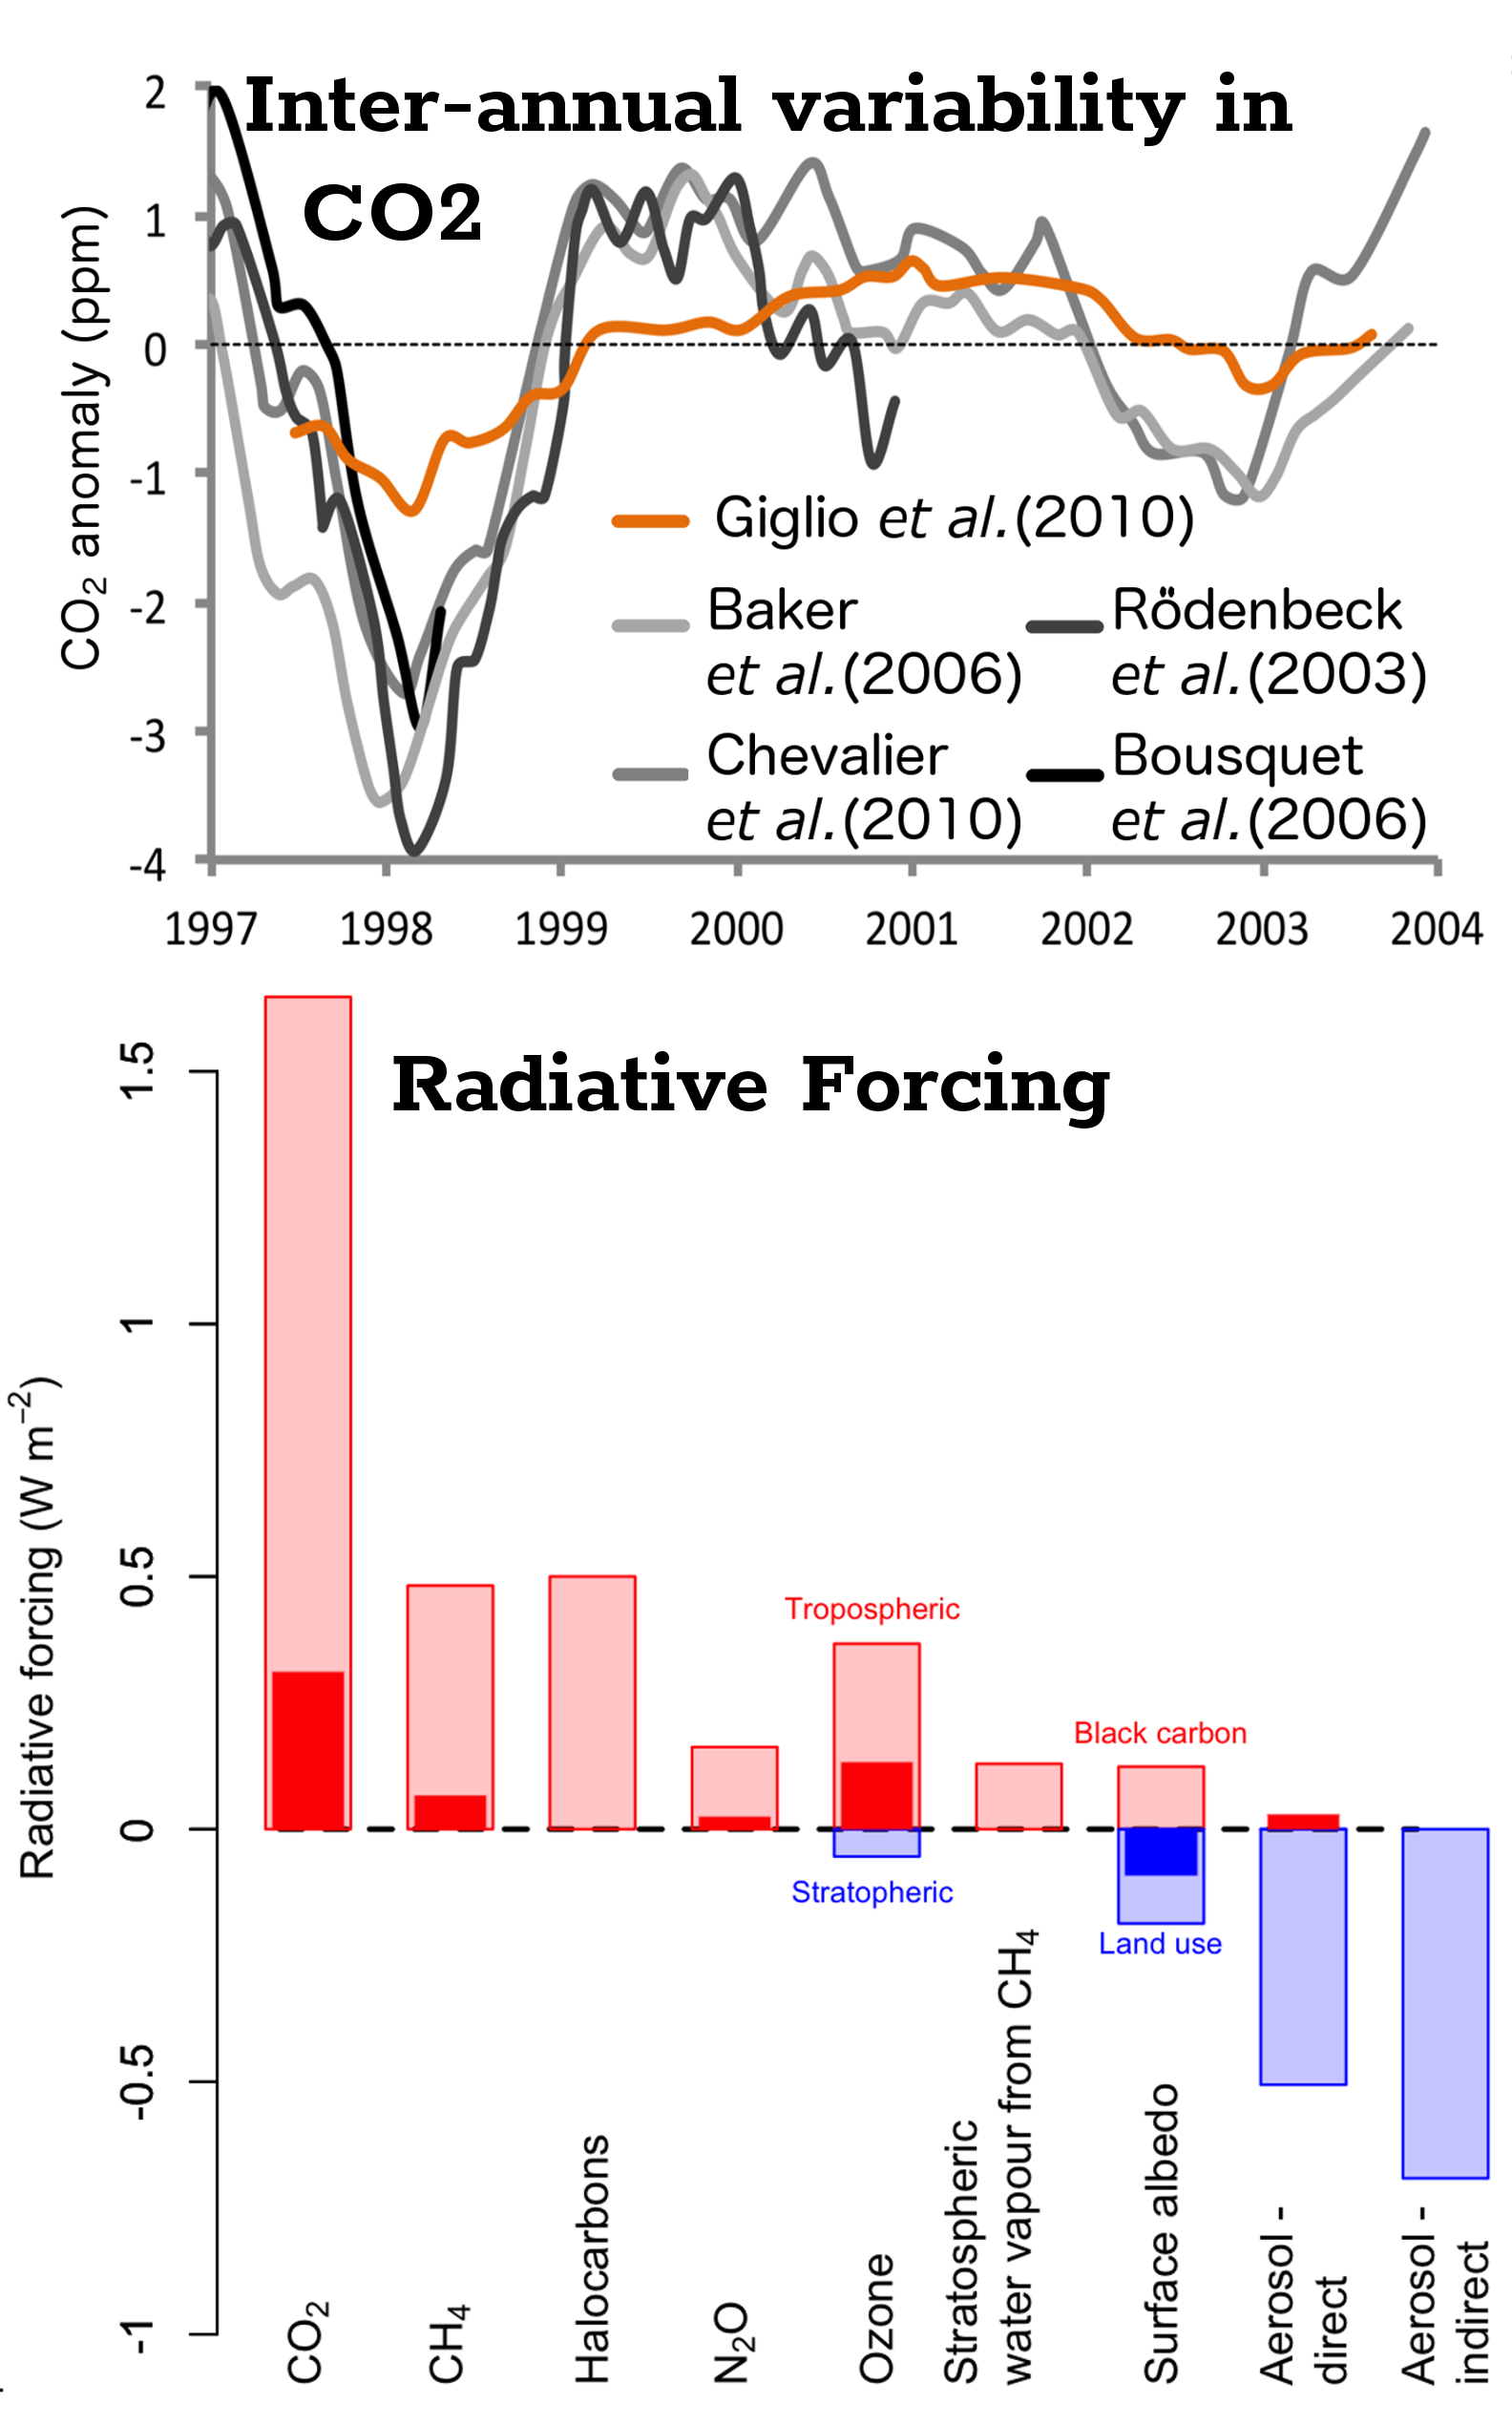
\includegraphics[width=4.80cm]{images/fireImportance}%images/unimodal/p\x.png}
			};}
		
		\only<2-3> {
			\node[anchor=south west,inner sep=0] (image) at (0cm,2cm) {
				\adjincludegraphics[trim={0 {.53\height} 0 0},clip, width=12cm]{images/firePerBiome}%images/unimodal/p\x.png}
			};}
		\only<3>{
				
			\draw[blue, line width = 0.25mm] (5.2,5.65) -- (6.5,5.65) -- (6.5,6) -- (5.2,6) -- (5.2,5.65);
			
			\draw[blue, line width = 0.25mm] (5.6,4.8) -- (6.5,4.8) -- (6.5,5.3) -- (5.6,5.3) -- (5.6,4.8);
			
			\draw[blue, line width = 0.25mm] (9.5,4.5) -- (10.5,4.5) -- (10.5,5.0) -- (9.5,5.0) -- (9.5,4.5);
			
			\draw[blue, line width = 0.25mm] (2.7,4.8) -- (3.5,4.8) -- (3.5,5.3) -- (2.7,5.3) -- (2.7,4.8);
		}		
		
		\visible<4> {
			
			\node[anchor=south west,inner sep=0] (image) at (6.5cm,0cm) {
				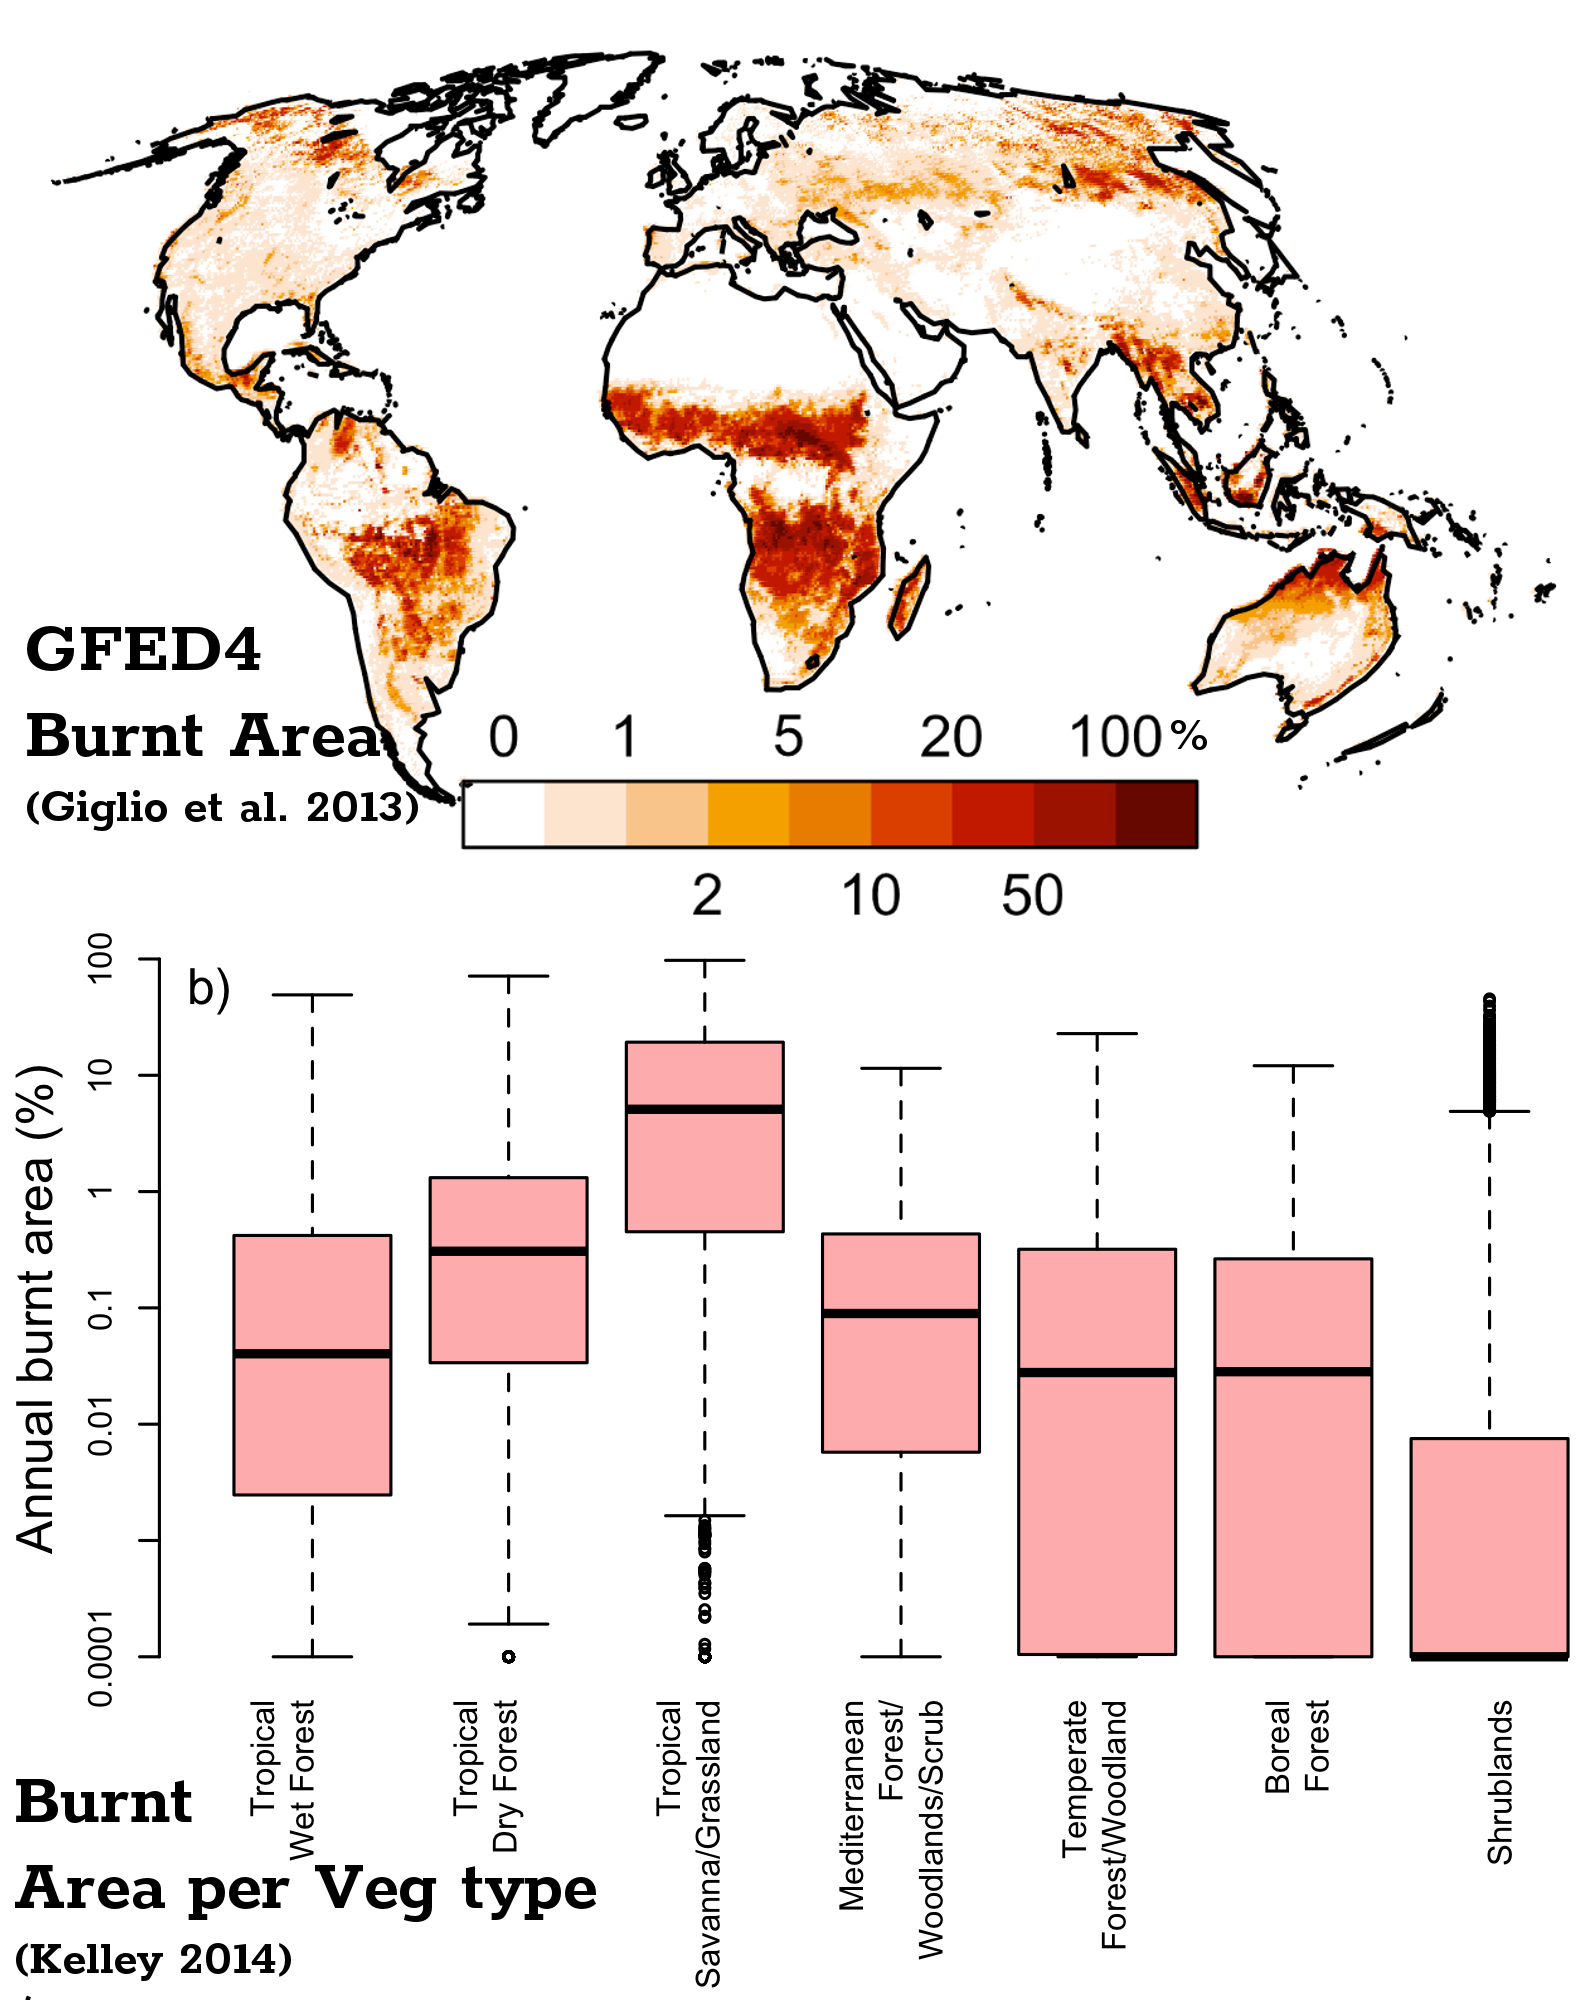
\includegraphics[width=6.05cm]{images/firePerBiome}%images/unimodal/p\x.png}
			};}
		\end{tikzpicture}
	\end{textblock*}
	
	%Make clear we are talking about burnt area
\end{frame}

\begin{frame}[label = intro]
	\frametitle{Fire and carbon}
	%\framesubtitle{Is it Ignitions? Is it people?}
	
	\begin{textblock*}{14cm}(-0cm ,1.3cm)
		\foreach \x in {1, 2, 3, 4, 5, 6} {
			\only<\x> {
				
				\includegraphics[width=10cm]{images/fireCarbonBalance/pp\x.png}
			}
		}
		
	\end{textblock*}
	
	
\end{frame}

\begin{frame}[label = intro]
	\frametitle{fireMIP}
	\framesubtitle{Fire Modelling Inter-comparison Project}
	
	\begin{textblock*}{14cm}(-0.0cm ,1cm)
		%\begin{tikzpicture}
			\foreach \x in {1, 2, 3, 4, 5} {
				\only<\x> {
	%				\node[anchor=south west,inner sep=0] (image) at (0,0) {
						\includegraphics[width=11.7cm]{images/fireMIP/pp\x.png}
	%				};
				}
			}
	\end{textblock*}
	\begin{textblock*}{5.5cm}(7.2cm ,2.5cm)
	%		\node[anchor=south west,inner sep=0] (image) at (6.5cm,0cm) {
				\begin{itemize}
				
					\visible<2->{\item Benchmark overview}
					\visible<3->{\item Focus on JULES performance \& fire controls}
					\visible<4->{\item Diagnose seasonality performance}
					\visible<4->{\item Explore missing anthropogenic processes}
					\visible<5->{\item Other fireMIP evaluation we could take advantage of}
				\end{itemize}
	%		};
	%	\end{tikzpicture}
	\end{textblock*}
			
			%	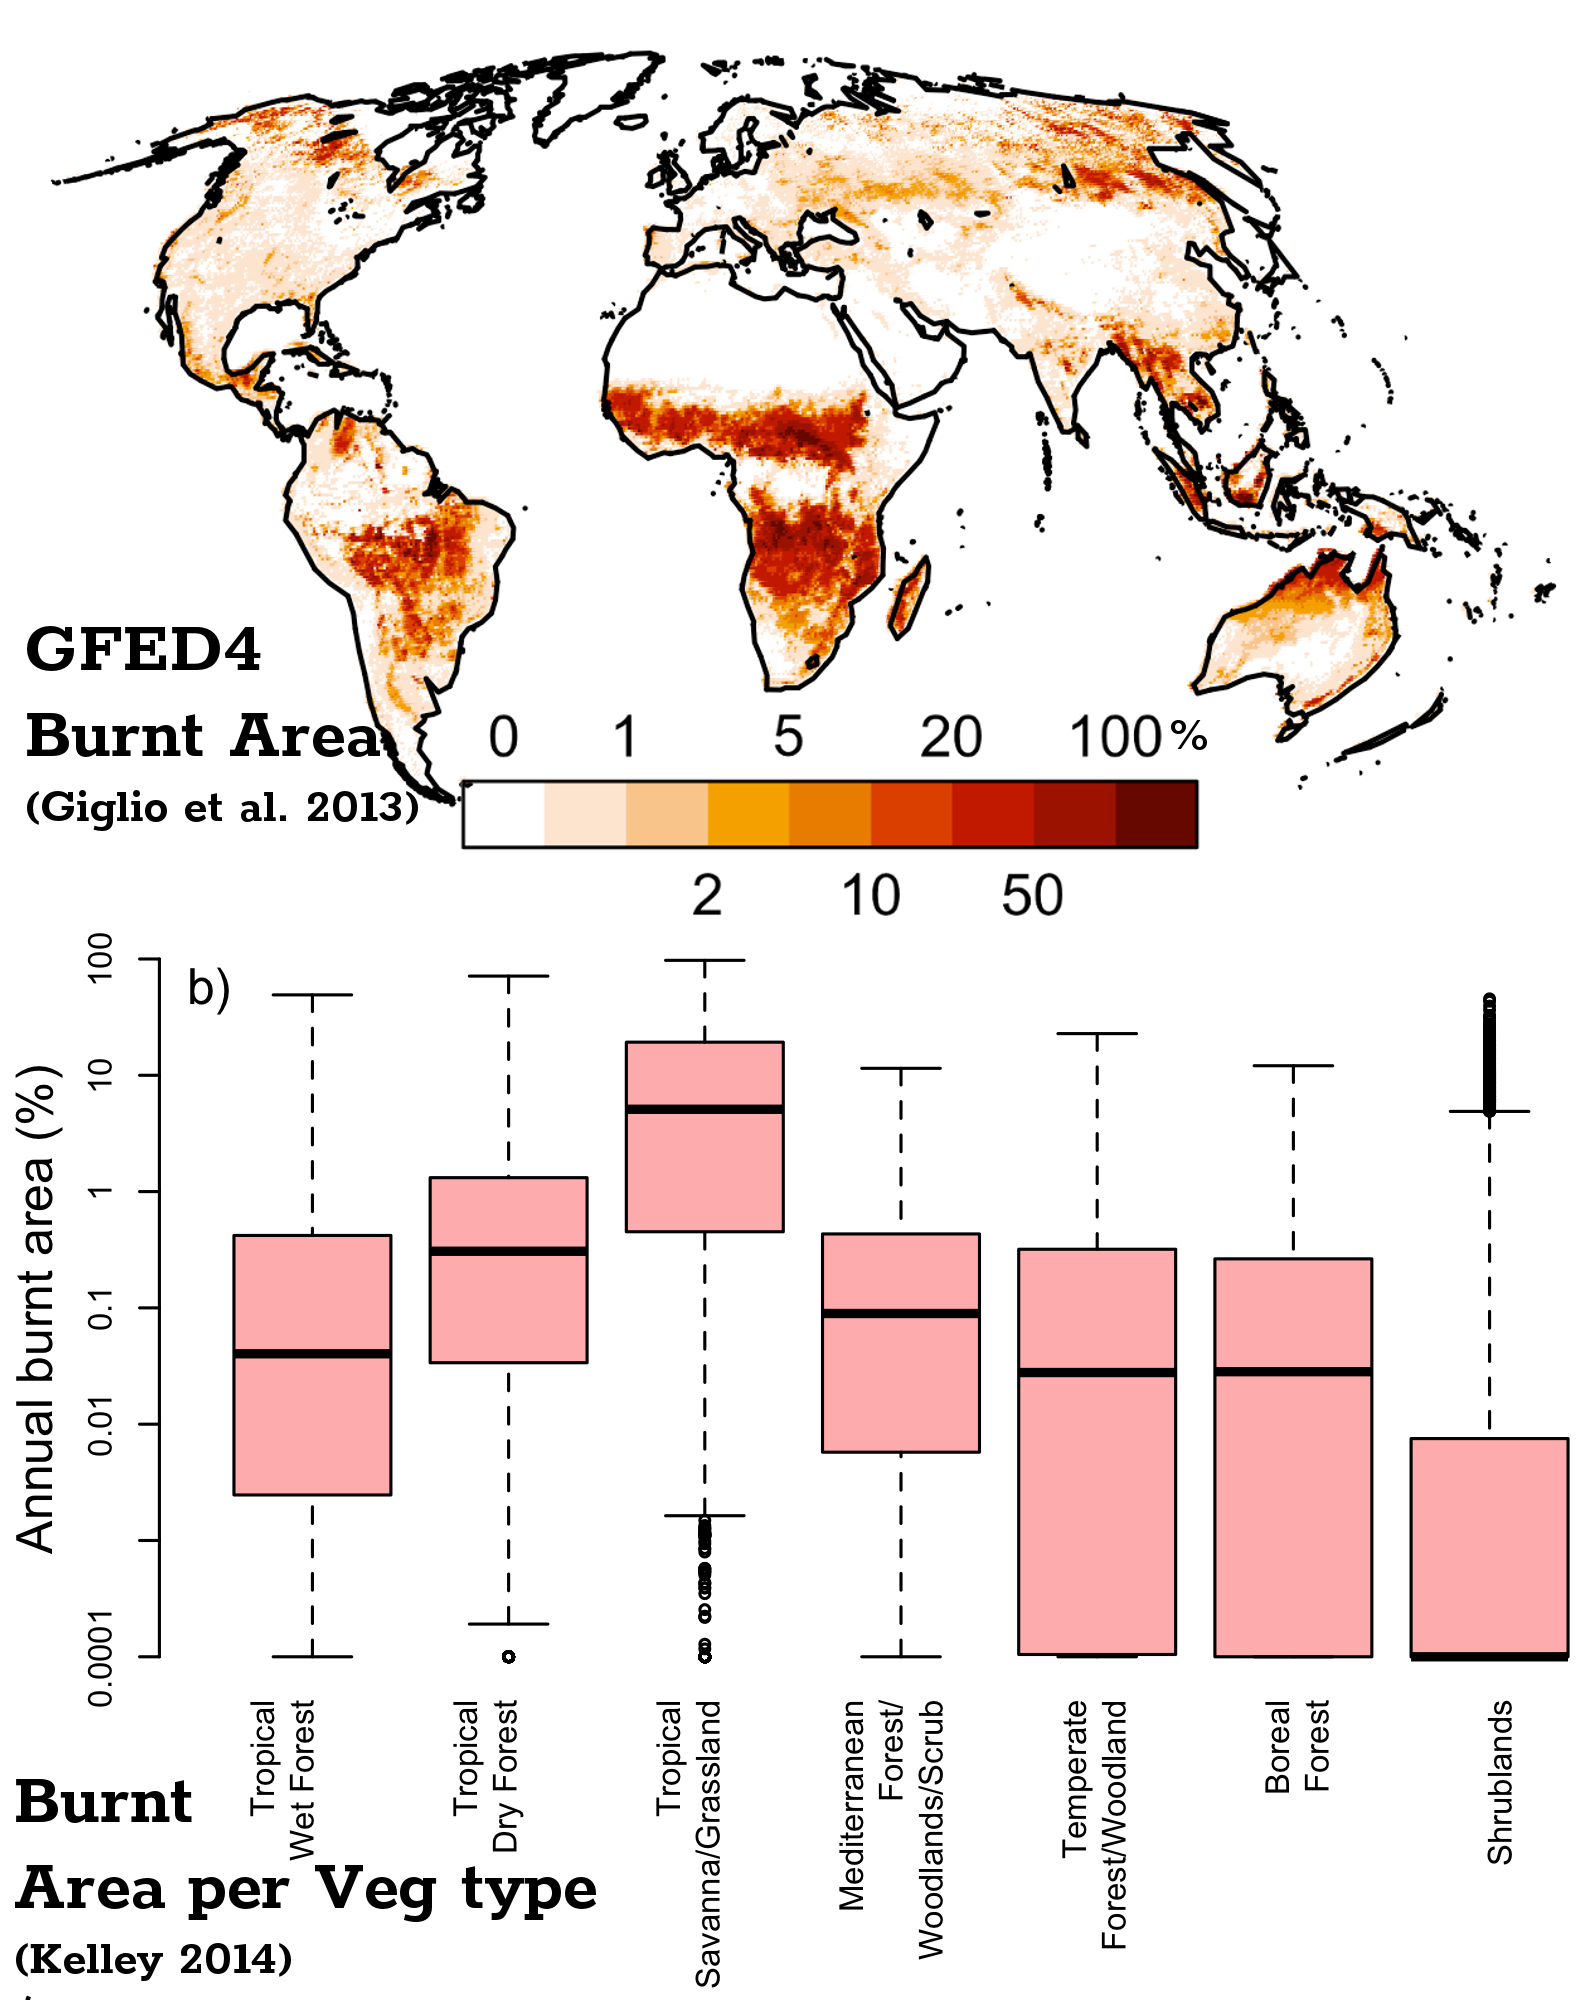
\includegraphics[width=6.05cm]{images/firePerBiome}%images/unimodal/p\x.png}
			%};
	%}}
\end{frame}

%\begin{frame}[label = intro]
%	\frametitle{fireMIP}
%	\framesubtitle{Fire Modelling Inter-comparison Project}
%	\begin{itemize}
%		%\huge{
%			\only<1-4> {
%				\visible<1->{\item Little agreement between models simulated fire}
%				\visible<2->{\item No systematic inter-model comparison of fire or fire drivers}
%				\visible<3->{\item No comparison of different model hindcasts and future projections, and their sensitivity to different drivers}
%				\visible<4->{\item fireMIP setup to address this}
%            }
%	        \only<5-> {
%		        \visible<5->{\item fireMIP model overview}
%		        \visible<6->{\item fireMIP benchmarking system}
%		        \visible<7->{\item Multi-model results}
%		        \visible<8->{\item JULES-INFERNO model performance}
%		        \visible<9->{\item Process evaluation}
%	        }
%	\end{itemize}
%\end{frame}
